%Tutkimusaineisto ja -menetelmät
% vai: multi-view stereo rig implementation
\section{3D scanning rig implementation} \label{sec:implementation}

Now that the background has been introduced, the practical part of this thesis follows.
Specifications for a 3D scanning rig are given, and different off-the-shelf camera types are compared more in depth.
Suitable cameras for the task are then selected and described, with the decisions on mechanical construction.
Control software for the rig is developed, and a survey is given on the readily available offering of reconstruction software.
Tests of the built system are given in Section \ref{sec:experiments}.

\subsection{Functional specification} % {{{

Constraints on the rig were specified in loose terms, leaving much work on the background study.
Desirable properties of the system were given as:

\begin{itemize}
	\item Ease of use and practicality: the user should not need to know the implementation details (hardware internals or algorithms) or to have programming skills to calibrate the system and acquire a 3D scan; scanning should be as simple as pressing a button
	\item Flexibility: for research purposes, many subjects should be possible to scan
	\item Mobility: the system should not rely on affixing fixtures on the walls or the ceiling, for example
	\item Detail: high resolution should be used for achieving data for state-of-the-art algorithms
	\item 3D and 4D: both static surface reconstruction and variations in geometry over time should be possible to scan
	\item Open design: by documenting the rig well and selecting readily available generic components, a similar system could be built if there was such a need, and the already built system could be easily extended
	\item Reasonable price: the total budget of all hardware and software combined should not exceed 10~000 EUR.
\end{itemize}

A general-purpose reconstruction rig has many practical matters to consider; some decisions can be judged by the understanding based on the pure mathematical background, while others are purely based on practical reasons.
Flexibility for arbitrary subjects means, among other interests, that the rig should be adjustable enough by means of camera positions and viewing directions.
Distance to the photographed target should not be too short in order to not annoy human subjects, but a too large setup may be difficult to build and needs a lot of space on the floor.
When capturing video, the frames should be synchronized among cameras as described in Section \ref{sec:video}, which might not be perfectly possible with consumer hardware.
A mobile rig should be light enough to carry, set up, and reconfigure for new subjects, but it should be rigid enough to give proper quality pictures and hold its calibrated configuration.
Cameras are chosen among pocket cameras, system cameras, and industrial machine vision systems currently in the market.

% }}}

\subsection{Camera comparison} \label{sec:cameracomparison} % {{{

Section \ref{sec:cameratypes} presented the typical properties of different camera categories in general, and compared them to technical requirements.
In this section, the focus is more on the feasibility of the properties on reconstruction, and on selecting a collection of feasible cameras fitting in the budget.

\paragraph{General problem statement}
Small subjects in the range of a metre or less introduce concerns in shallow depth of field, forcing the lens aperture small, and consequently, requiring bright lights or slow shutter speeds.
More sensitive sensor would require less light, but depth of field decreases as the sensor size increases.
As the capture environment will be a clean indoor space and the cameras will mostly be controlled remotely, features usually important to photographers such as weatherproofing or user interface are not considered.
Reliability on configurability and controllability is considered important.
Cheaper cameras fit more into a budget, offering more coverage of the subject, but they might not be properly controllable.
External shutter release mechanisms have been researched more on DSLRs than compact cameras, and most compacts do not have one;
the manufacturers do not provide official specifications of the release connector pinouts, but they have been reverse-engineered for many models by individual tinkerers.
Machine vision (MV) cameras, in contrast, support only external shutters.
Zoom-only lenses, lack of raw image output, remote configuration and manual modes, and slower processing speed leave cheaper compact cameras out of the comparison practically altogether.
More expensive models do have comparable features, and their prices rise into the same range as with DSLRs that are more understood.

\paragraph{Previous work}
Canon DSLRs have been used previously on commercial static capture setups \cite{ir-ltd,ten24,capturelab,agisoftforum}.
Many hobbyists in the Agisoft forum suggest a Canon or Nikon DSLR. \cite{agisoftforum}
Commercial video capture setups may use specialized machine vision devices and hardware-accompanying or customized software for image capture and reconstruction. \cite{TODO}
Also standard commercial video cameras have been used \cite{bradley2010high}, but their resolution is limited.

\paragraph{Specialized hardware requirements}
Whereas self-contained consumer devices are not designed for and do not support any additional devices for capturing the imagery, machine vision devices need several high performance computers for reliable multi-camera capture because of the lack of local storage.
While each camera outputs easily 1 Gbit/s worth of raw data or more (Equation \ref{eq:gigabit-transfer}), a common desktop computer and one additional hard disk per camera is needed if the capture is long enough and does not fit in a computer's RAM, increasing the system cost and complexity.
%For a small number of cameras, existing buses on a PC might be enough, but a larger number requires even more bandwidth.
Best mechanical hard disks currently have sequential write speed that just exceeds 1 Gbit/s \cite{wdtaijotain};
newer solid-state drives (SSD) generally are two to four times faster. \cite{todo}
For covering all the bandwidth, expansion cards would be needed per camera, count depending on the camera protocol.
Most PC motherboards can accommodate only a few cards, requiring several PCs.

Transfer speeds given by specifications and theoretical maximum frame rates for typical 12-bit raw full-HD frames are listed in table \ref{tab:busspeeds}; achievable rates would be less depending on bus overhead.
In contrast, best Compact Flash (CF) cards, used in professional consumer DSLRs, can write at approximately 150 MB/s, while cheaper Secure Digital (SD) cards reach 90 MB/s, but camera bus drivers usually only achieve 20-40 MB/s. \cite{todo} % TODO canon, magic lantern, uhs-i

\begin{table}[h]
	\centering
	\begin{tabular}{l l l}
		Bus type & Maximum theoretical speed & Naive max.\ frame rate\\
		\hline \\
		USB 2.0 & 480 Mbit/s & TODO\\
		USB 3.0 & 3.2 Gbit/s & TODO\\
		Camera Link & 5.44 Gbit/s? & TODO\\
		FireWire & 3.2 Gbit/s? & TODO\\
		GigE & 1.0 Gbit/s & TODO\\
		SD card with UHS-I & 832 Mbit/s & TODO\\
	\end{tabular}
	\caption{Bus speeds and corresponding frame rates}
	\label{tab:busspeeds}
\end{table}

\paragraph{Preferred properties}
A camera is required to have several properties, and the system as a whole must be taken as a global optimization problem, since some properties conflict each other.
In detail, the technical camera features that should be considered are described in Section \ref{sec:image-acquisition} and features that vary among different cameras are listed below.

On image quality:

\begin{itemize}
	\item CMOS/CCD sensor. CMOS suffers from rolling shutter in video mode, while global-shutter CCD is more expensive and rare in larger formats.

	\item Resolution and sensor size. Higher resolution covers more detail, until the optical limits of the system are reached. A larger sensor has larger pixels, and is thus more sensitive to light and results in lower noise and lower required exposure time. On the other hand, at an equivalent subject distance, a deeper DOF is achieved with a smaller sensor.

	\item Low noise. Sensor noise degrades image quality in general, adds error to subpixel position estimation and complicates correspondence search, etc.

	\item Dynamic range, i.e. bit depth of the processing pipeline. Whereas JPEG pictures have only 8 bits per color channel, DSLRs and industrial cameras use more, often 12 or 14 bits per pixel in raw format, that contains the color filter array effects before interpolation. Postprocessing without reconstruction can use the added color resolution.

	\item Lens quality. High sensor resolution is only useful if the lens is sharp enough, and color aberrations degrade image quality in general. Fixed focal length lenses have less moving parts and hold their calibration better. The performance of good lenses is usually given as an MTF, or modulation transfer function, describing the best possible contrast.
\end{itemize}

On practical matters affecting image quality:

\begin{itemize}
	\item Optical stabilization works by moving a glass element inside the lens or the sensor itself, effectively moving the image on the sensor, having also an effect on calibration.

	\item Dust reduction, if enabled for some consumer cameras, is typically implemented as high-frequency vibration of the sensor on camera startup. Moving the sensor might result in small calibration problems.

	\item Shutter lag. Lag measured between ordering the camera to take the picture to the actual moment where exposure starts should be consistent, and preferably small.

	\item Video frame rate, resolution, and compression. Cameras that support a raw format only use raw for still pictures and compress the video, as raw video is unnecessary in the consumer market and uses lots of space. For image processing, each frame should be as little compressed as possible. Some DSLRs support writing only full keyframes instead of predicted frames, resulting in higher quality and file size.

\end{itemize}

On practical matters affecting usability:

\begin{itemize}
	\item Lens features. While photography lenses typically support automatic focusing, MV lenses only have manually adjustable or fixed-distance focus. Of photography devices, compact cameras feature a non-changeable zoom lens, while system cameras feature interchangeable lenses.

	\item Continuous shooting rate, or the speed at which full-size pictures can be taken. Controlled by many factors, on consumer cameras, image processing speed and memory card write speed have most effect, and on MV cameras, the bus speed typically limits the rate and sensor speed is selected based on it.

	\item Configurability. Aperture, shutter speed and others should be manually controllable remotely, and repeatable without automatic features.

	\item Remote trigger. Practically all DSLRs have wired or wireless remote shutter releases; some machine vision cameras have optionally an external logic-level trigger input in addition to one that is set by the protocol in the data bus. Some protocols may have global commands to send throughout a group of cameras. (FireWire?) Otherwise, software trigger suffers from sporadic jitter from operating system and protocol non-determinism.

	\item For consumer cameras, USB read speed supported by the camera. Retrieving saved image or video data takes less time for faster interfaces.

	\item External flashes. Practically all system cameras can be wired to an external flash unit; only some compact cameras support this. Industrial cameras are always externally triggered, some supporting a separate independent signal and some via the transfer bus.

	\item External power supply. Not needing to charge batteries adds value to the ease of use.

	\item Weight and size. A smaller and lighter camera requires less bulky support structures.

	\item Price. With a fixed budget, cheaper cameras can cover a larger area of the subject at a time because more cameras fit in the budget.

	\item Availability. For an easily replicable system, it should be simple to purchase the hardware.
\end{itemize}

In general, good technical properties are deep depth of field, light sensitivity, high resolution, and short distance to the subject.
Practical features also count, such as availability of external power supply instead of batteries.

All the properties should be looked as a whole; especially large pixel count does not necessarily imply better pictures if the optics is not good enough.

Prices for compact cameras that have the required features go up to the same price range as DSLRs or even higher, i.e. 500 EUR and up.

Having a much smaller production rate than larger manufacturers that target consumers (such as Canon, Nikon, Pentax or Sony), MV cameras have a broad price range from a few hundred euros to thousands, well correlated with pixel count and frame rate.
Lens prices for the C-mount optics used by MV are moderate, at around 200-300 EUR.
Properties of MV hardware is typically better specified than that of consumer devices, but prices of complete systems are an order of magnitude higher.

%The price of professional video cameras leaves them out of the comparison, them being an order of magnitude more costly than average consumer devices.

% }}}

\subsection{Selected cameras} % {{{

A number of compacts, system cameras, and machine vision cameras were reviewed.
In this section, the selected key parts are described in detail.
Precise information on all hardware used can be found in appendix \ref{app:hardwareused}.

In general, machine vision cameras were considered overly expensive, although they perform best in synchronized video and output the frames in lossless raw format.
Compact cameras do not have significant advantages over DSLRs, when comparing models where both have comparable required features, such as remote controllability and external shutter release options.
{ \color{red} FIXME: actual table of some sample models somewhere here. }
A DSLR is a good choice for still photos because of moderate price compared to image quality, and availability of usable software and best range of accessories.
Video recording is notably worse than with machine vision that can produce higher resolution, raw data, and synchronized output;
because of a price difference of almost an order of magnitude for cameras having a comparable resolution, it was decided to leave high-performance video tracking as a minor feature, and concentrate on static subjects.
Canon was chosen over others because of firmware customizability \cite{magiclantern}, previously acquired personal knowledge of the manufacturer, well specified remote control abilities \cite{canonedsdk}, and previously proven work using the same maker \cite{ir-ltd,ten24,capturelab,agisoftforum}.

\subsubsection{Canon EOS 700D DSLR}

\simplefig{h}{%
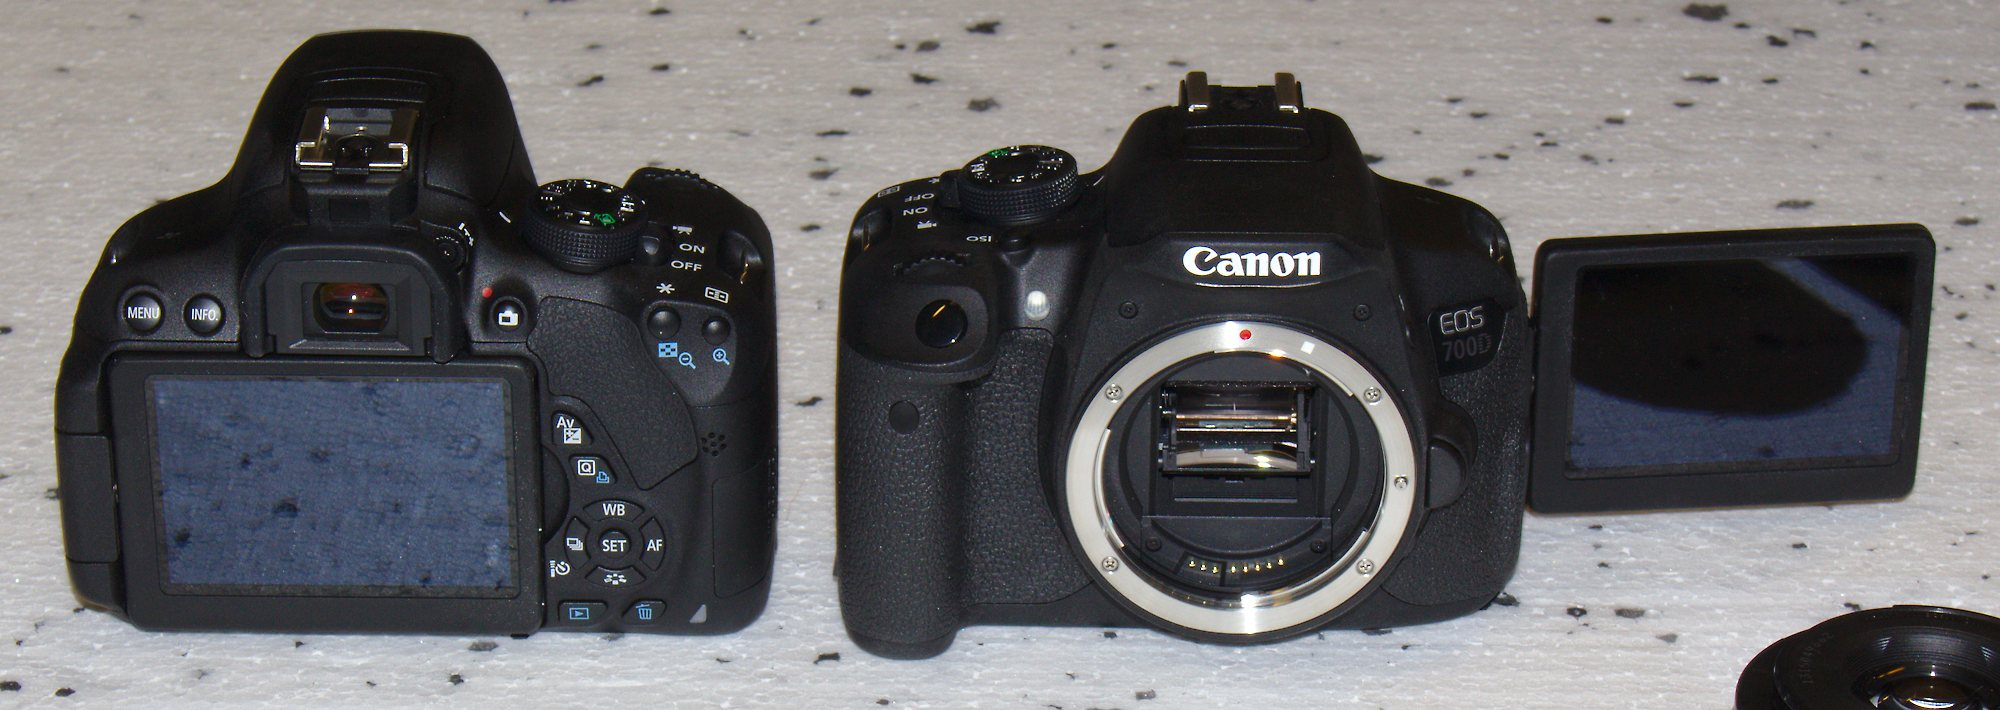
\includegraphics[width=0.8\textwidth]{eos700d}
}{fig:eos700d}
{Canon EOS 700D DSLR camera body}

Canon EOS 700D body, also known as the Rebel T5i, introduced in 2013, is the newest of Canon's consumer range DSLRs, with a price at about 600 EUR at the point of writing.
Key features are shown in Table \ref{tab:eos700dfeatures}.
It was decided to build the rig around nine of them.
The front and back view of the camera are depicted in Figure \ref{fig:eos700d}.

\begin{table}[h]
	\centering
	\begin{tabular}{l l}
		Sensor type & CMOS\\
		Sensor size & APS-C 22.3 x 14.9 mm\\
		Pixel size & 4,3 x 4,3 $\text{\si\micro m}$\\
		%CoC span at 0.019 mm & 4.4 pixels\\ % (FIXME move to lens)
		Image resolution & 5184 x 3456 pixels (17,9 million) \\
		Processor & Canon Digital Imaging Core (DIGIC) 5\\
		Bits per pixel & 14\\
		Continuous shooting speed & 5 FPS\\
		Video mode & 1080p in 30 FPS or 720p in 60 FPS\\
		Max write speed & $\approx$ 40 MB/s
	\end{tabular}
	\caption{Canon EOS 700D key features}
	\label{tab:eos700dfeatures}
\end{table}

\paragraph{Properties}
Relatively large pixel count combined to a good lens captures high-resolution detail.
The sensor's pixel size is not unnecessarily small but not as large as in full frame DSLR cameras.
%Dynamic range with 14 bits per pixel is relatively large; most reconstruction programs use 8-bit images, though.
% raw images useful for manual image enhancement
The 5 FPS continuous speed for full-size images can be used for testing high resolution motion, but the video abilities are also reasonable.
The quality can be tweaked with firmware modifications and raw video recording is also possible, at reduced resolution limited by storage speed. \cite{magiclantern}
The sensor is labeled ``Hybrid CMOS'', a new Canon's technology that embeds phase-detection autofocus pixels in the sensor for fast continuous autofocusing in video mode.
A number of pixels is missing color sparsely around the middle of the sensor and are interpolated; they only introduce artifacts in raw video.

%Older models of the same product line can still be found in the market, such as 650D or 600D.
%700D has a newer processor and thus faster processing speed, faster memory card controller and others.
Resolution of the sensor has stayed same since the EOS 550D, introduced in 2010.
At the same time, also cheaper new models are available, such as the EOS 1200D; at a reduced price, less processing power is provided, resulting in slower operation but otherwise the cameras share mostly same features.
The more expensive professional cameras vary mostly by processing speed and build quality.

\paragraph{Storage}
The camera uses Secure Digital (SD) memory cards for mass storage, supporting the UHS-I standard (Ultra High Speed).
Maximum write speed has been found experimentally to be approximately 40 MB/s \cite{magiclanternforum}.
A class 10 UHS-I memory card was selected; manufacturer claims 45 MB/s write speed.

\paragraph{Conveniences}
The camera also features a tilting LCD screen that has provided to be useful when looking the camera from the front.
Additionally, AC power adapters were chosen to operate the cameras without the need for charging batteries.
Canon sells adapters that plug in the camera's battery holder, providing continuous power at the expense of an additional cable per camera.
For wireless remote shutter, the camera natively supports an infrared remote controller that must be pointed towards the camera from the front.

% flashguns

\subsubsection{Canon EF 50mm f/1.8 II}

Canon's EF-mount 50mm f/1.8 II lens (priced at about 110 EUR), shown in Figure \ref{fig:canonef50mmlens} is well known for its excellent image quality at a low price.
The lens was introduced in 1990.
The 50 mm focal length with the crop factor of 1.6 of the camera body provides a good shooting distance for the purposes of this work.
Like most lenses at this focal length, the lens is nearly distortion free.
Despite the poor plastic build quality, its glass is of very high quality and it is well known as one of the best portrait lenses for photography.
The lens changes between autofocus and manual focus modes with a mechanical switch, and the focus ring in manual focus mode is loose enough that it might need to be locked with tape if left on for a long time shooting to hold its position for a calibrated setup.

At a distance of one metre $d = 1$ m, the sensor size of $s_x \times s_y$ = $22.3 \times 14.9$ mm and $f = 50$ mm focal length, the area that fits in the frame is $a_x \times a_y$:

\begin{align} \label{equ:areasize} \begin{split}
	a_x &= s_x \times \frac{d}{f} = 22.3 \text{mm} \times \frac{1 \text{m}}{50 \text{mm}} = 446 \text{mm}\\
	a_y &= s_y \times \frac{d}{f} = 14.9 \text{mm} \times \frac{1 \text{m}}{50 \text{mm}} = 298 \text{mm}
\end{split} \end{align}

which is easily seen from similar triangles with a common corner.
From Equation \ref{eq:dof}, the depth of field at this setting is about 16 cm for a f-number of f/11, or 20 cm for f/14, at circle of confusion of 0.019 mm, a reasonable depth for the given area size.

\simplefig{h}{%
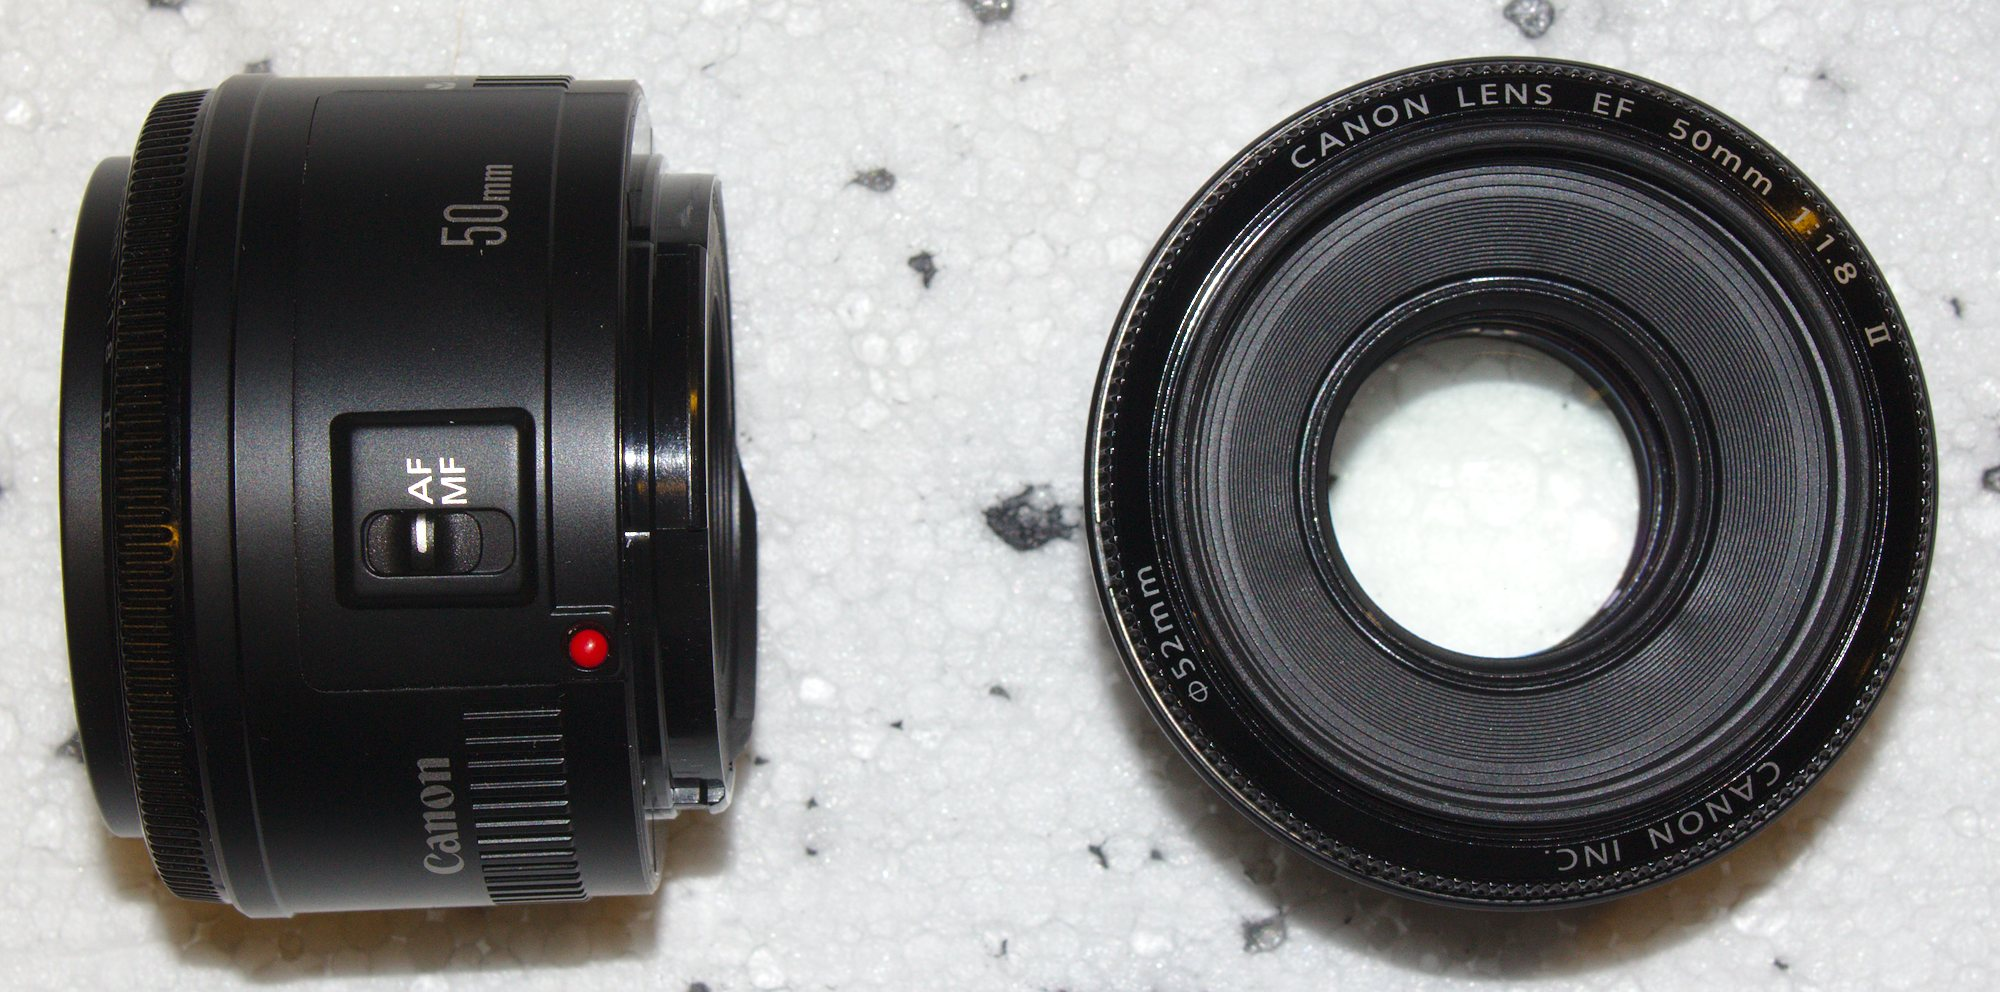
\includegraphics[width=0.8\textwidth]{canon50mmlens}
%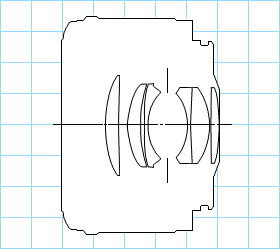
\includegraphics[width=0.4\textwidth]{canonef50mm-2}
}{fig:canonef50mmlens}
{Canon EF 50mm f/1.8 II, a fixed focal length lens with manual focus and autofocus}

\subsubsection{Magic Lantern}

An important consideration was the ability to use the third-party Magic Lantern (ML) firmware add-on;
it was originally developed for tools and improved user interfaces for video recording, but has been extended for numerous other features too.
It was installed on each camera in the rig.
Firstly, it provides experimental support for raw video recording, easier remote triggering for video, and other hacks;
additionally, being open source, it can be modified for any custom purposes, such as multi-camera synchronization aids, if necessary.
It is a separate native program for the ARM-based DIGIC processor, and runs in the camera alongside the original firmware, loaded from the memory card, using the same operating system and configuration menus. \cite{magiclantern}
A screenshot of a menu grid displaying some of the additional functions is shown in Figure \ref{fig:ml-menu}.

ML is installed on a memory card, and it does not make permanent changes to the camera's original firmware.
Still, being third-party software based on reverse-engineering efforts, there is a small risk of unexpected instability.
ML has an active user forum, a wiki, and an automatic software build system for releasing nightly testing versions.
As an open source project developed in a distributed fashion, it suffers from inconsistent documentation and coding style, and is occasionally best examined by reading source code, written in the C programming language.
No stable release is offered for EOS 700D yet, but the unofficial testing version has been long in use by the community. \cite{magiclantern}

\simplegfx{h}{0.6\textwidth}{ml-menu}{
	Magic Lantern grid menu in movie mode, showing a subset of its features.
}

% }}}

\subsection{Hardware construction} % {{{

The cameras need additional support structures for mounting.
A trivial solution would be a tripod for each camera, which would not allow stacking the cameras vertically, though.
Two main methods were considered; they are described below.

\subsubsection{Mechanical options}

With flexibility and mobility as requirements, the system should be built of removable parts that need no modifications to the environment, such as screwing bolts to nearby walls.
The separate parts should be small enough for transportation, but large enough for rigidity and build simplicity.
Each camera should be able to turn at least in landscape and portrait mode to fully utilize the picture frame for portrait subjects, such as human faces.

Two different major designs were considered: a hinged frame consisting of industrial aluminium profile system, or individual tripod stands available in most photography stores meant for supporting audiovisual equipment.
For connecting the cameras, a custom profile could make use of also custom built parts; also, photography stores sell screws and clamps meant for connecting cameras, lights and other hardware.

Extruded aluminium profiles such as those by MiniTec, Item or Bosch Rexroth consist of rectangular tube with a T-shaped slot running along each side for screws, sometimes called T-slot systems.
%The profile systems are commonly used in assembly lines and other automation installations in factories, but also in smaller assemblies
Mechanical dimensions vary by manufacturer but most supply a large catalog of connection brackets, hinges, screws etc.\ that allow much flexibility in the frame design.
A hobbyist-purposed manufacturer OpenBuilds targets open source projects, such as 3D printers and CNC routers.
The cost of such profile is around 10-20 EUR/m, with varying prices for connection pieces; availability varies by supplier.

Ready-made light or speaker stands come in a variety of sizes and share a common design with an extendable center rod and three legs.
Typical light stands have an universal mount in top end of the rod for fastening a lamp.
Speaker stands typically share a similar standard; in general, they are also heavier and thicker to support a larger mass.
Most photography and audio/video studio stores offer a variety of light and speaker stands.

A custom aluminium profile system would have its benefits in rigidity and positional flexibility, because it could be built in any shape.
On the other hand, one rigid shape is more difficult to modify when such a change is needed.
Standard light or speaker stands are attractive because of their availability in normal stores.
They also can be moved around, which also means more work in configuring the camera poses again.
A stand consisting of mostly round rods lacks flat surfaces and slots that could be used for fastening parts together.
For that purpose, special clamps and ball heads are sold separately.

Machine vision cameras do not generally use the same tripod screws aimed for consumer market, but are screwed on the frame with custom bases.

\subsubsection{Selected design}

The method of choice was to use ready-made, heavy duty lighting stands.
Millenium LST-310 (a brand by the Thomann music equipment store \cite{thomann}) is a sturdy three-legged lighting stand with a pole that can be extended several meters high.
Additionally, it has a rotating horizontal bar at the top.
Similar tripods were used in other projects in the same laboratory and they were found useful and rigid.
The relatively heavy weight (10 kg) makes the support structures steady. % FIXME weight
Four of these stands were bought, which should allow a moderate coverage around a subject. %and testing was done mostly with three, with three cameras in each.

For flexibility, each camera should be able to rotate in at least to horizontal or vertical pose, with arbitrary aiming position.
Manfrotto 494 ball heads were used for this purpose, connected to the tripod rod with Manfrotto 035 Super Clamps.
Figure \ref{fig:camconnection} shows a complete connection from a stand pole to a camera.

The total structure of all nine cameras divided in three supports (Figure \ref{fig:totalsetup}) takes up relatively little space, and is flexible enough to set up around any human-size subject or smaller.
The stands can be carried in bags and the more fragile parts are fitted in two cases shown in Figure \ref{fig:cases}.

Wires and power adapters are fastened to the stand legs in long-term use to reduce wires running on the floor.

\simplefig{h}{%
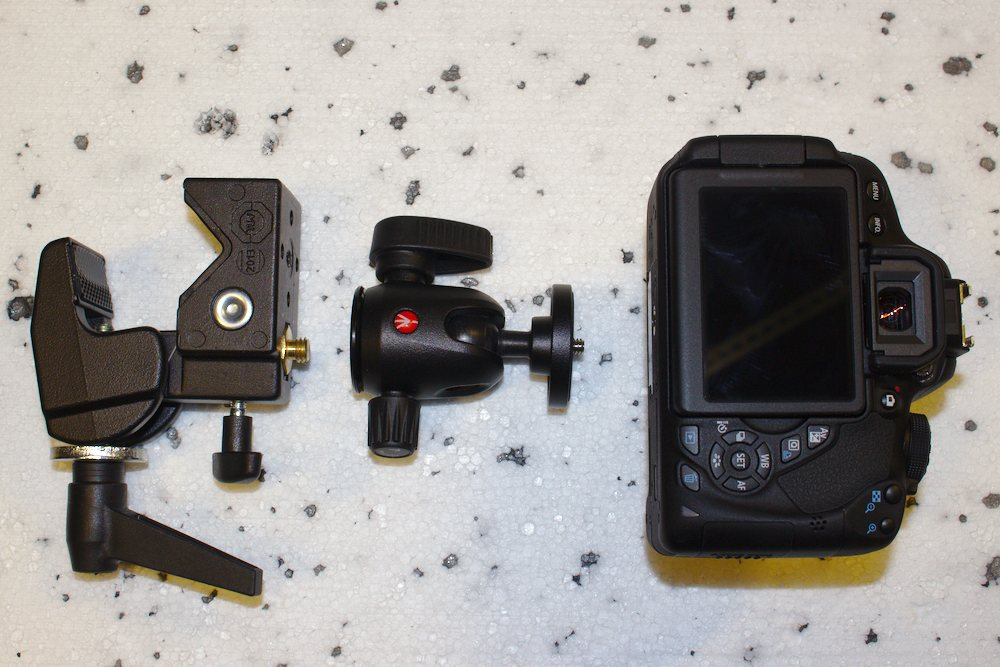
\includegraphics[width=0.45\textwidth]{connparts}
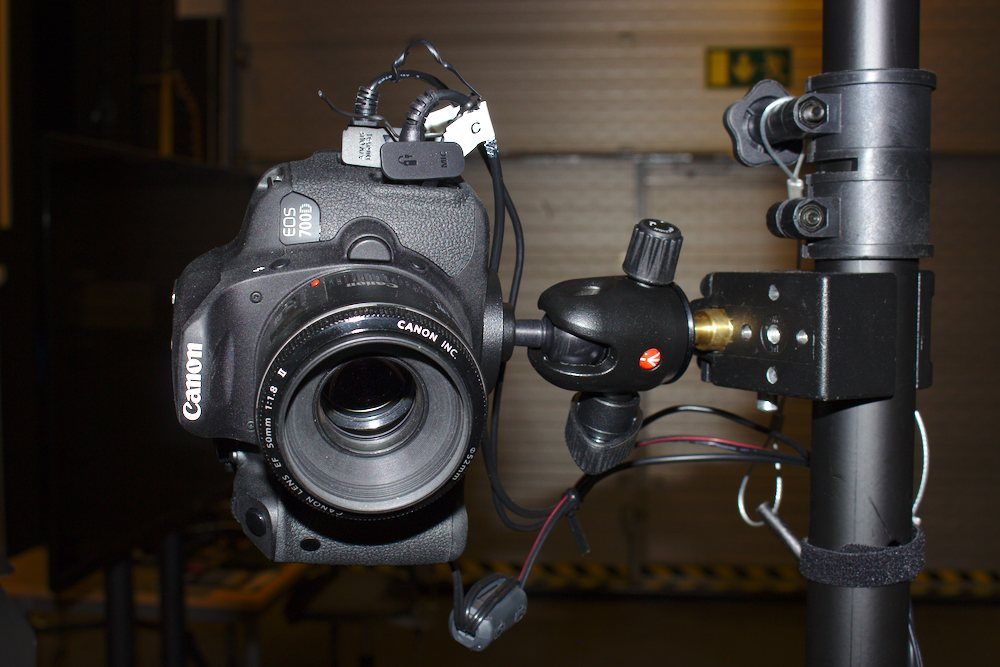
\includegraphics[width=0.45\textwidth]{camconn}
}{fig:camconnection}{
	Left: the Super Clamp, ball head, and a camera separately.
	Right: one camera connected to a pole and its wires.
}

\simplegfx{h!}{0.8\textwidth}{totalsetup}{
	Complete setup with cameras and spot lights for video recording.
}

\simplegfx{h!}{0.8\textwidth}{cases}{
	The fragile parts of the system fit in two equipment cases padded with soft foam rubber.
}

\subsubsection{Lighting}

An even lighting is necessary to capture the subject properly, as described in section \ref{sec:bg-lighting}.
Unwanted lighting artifacts include harsh shadows and sharp reflections.
Most shadows affect the scanned colors in an unwanted way, since the subject is to be relighted in a digital environment where shadows are formed artificially by calculating the brightness in every illuminated pixel separately.
Sharp reflections make reconstruction harder, since the position of the reflection depends on the viewing direction, making the appearance of the surface different in different views.

In still photographs, flash units bounced from white objects are a practical way to achieve a good lighting.
Typical flash units are either bounced away from white umbrellas sold for this particular purpose, or shot through a large and semitransparent cloth.
For video recording, either a continuous light source or a high-frequency stroboscope synchronized to the video frame rate would be needed.
Since the selected cameras do not support frame synchronization, a continuous light is necessary.

In the scope of this work, no lights were purchased, as readily available flash units and spot lights in the workplace could be used temporarily to evaluate the amount of light needed.
Two standard flash guns attached to the cameras were used for still photograph samples, and three studio spot lights were tested for video recording.
Detailed description on the lights is given in Section \ref{sec:samplesubjects}.

% }}}

\subsection{Remote shutter synchronization} % {{{

For a rig with possibly non-static subjects but an intended result of a still subject, the cameras have to be synchronized to record the subject at the same instance in time.
Photo synchronization was done with a remote mechanism provided by the camera, by driving the remote control of all cameras simultaneously.
However, a short light pulse of a flash unit typically synchronizes the cameras if the surrounding environment is dark, and the camera shutter synchronization has less strict requirements.
In video recording mode, the same remote wire can be used with 3rd-party firmware to start recording.

% }}}

\subsubsection{Canon remote trigger} % {{{

The selected Canon EOS 700D has an input port for focus trigger and shutter release, in addition to the integrated focus and shutter button.
The camera uses a standard 2,5 mm stero jack for connecting external remote controllers.
Wired and wireless electronic remotes are available in the market, but no standard devices for triggering several cameras arbitrarily are well available; some expensive wireless devices advertise support for multiple cameras using one shutter release, with no well defined latency.
Fortunately, the triggering method is widely researched among hobbyists; it is well enough documented in the internet.

The remote release jack is a three-contact connector, where one pin serves as a common ground, and connecting another pin to the ground triggers the camera's autofocus and metering, and the third pin releases the shutter when connected to the ground. \cite{docdiy}
The pins supply some current that flows back to the camera via the ground pin.
It is safer to separate the cameras from each other electrically instead of connecting the similar remote wires of all cameras together.
A commonly used method among the DIY community is to use opto-isolators to control each camera individually, isolated from the shared control circuit.

An opto-isolator provides a galvanically separated switch that can be used to electrically ``connect'' the release wire to the camera's ground such that no electrical signal path is shared between the cameras.
The switch is a phototransistor that is triggered externally by the light transmitted from a light emitting diode (LED).
Both the phototransistor and the LED are installed in an opaque plastic housing.
As an example, the opto-isolator device used in this work is shown in Figure \ref{fig:singleopto} next to the circuit it was used with.
The particular device works in open collector setting, exposing the collector pin that is left unconnected (``open'') and the emitter pin of the transistor.
Another common setting is a powered device that outputs a voltage signal from a power supply.

% }}}

\subsection{Universally synchronized multi-trigger} % {{{

By connecting each camera to a separate opto-isolator and driving all of them from same source, all cameras are triggered simultaneously in a safe fashion.
To fully automate the system, the trigger device should be connected to the computer that downloads the photos from the cameras.
Additionally, the cameras are enabled to shoot separately in addition to the synchronized simultaneous mode.

An alternative method in synchronization could have been one third-party wireless remote trigger per camera;
however, they are expensive (approximately 100 EUR per transceiver), may be not as consistent as a wired solution, and would require modifications to work connected to a computer.

\subsubsection{Microcontroller platform}

A microcontroller (MCU) is a tiny computer in a single, usually fingernail-sized package containing a microprocessor core, RAM, nonvolatile program memory and peripheral devices; all parts required to run a single user-defined embedded application typically with no general operating system.
The Arduino microcontroller board is a popular example.
The typical programming languages for microcontrollers are C and C++.
Communication on the host PC end of an USB connection, when supported, can be implemented in any language.

In this work, a microcontroller prototyping platform called Nucleo-F401RE by STMicroelectronics \cite{stnucleo} was used.
This platform has a built-in USB port for simple communication.

A MCU was chosen over e.g.\ a computer-controlled relay board because of its customizability and low price.
On one hand, such a device is more complicated to set up than a simple switch, but on the other hand, it can be programmed to sequence the cameras in any arbitrary order.
It can also be used to measure the shutter delay and the actual precise time when each camera takes the picture; each has small unpredictable variations.
When capturing moving targets, measuring this lag variation could be of interest.

\subsubsection{Hardware}

\simplegfx{h}{0.6\textwidth}{nucleo}
{STM32 Nucleo-F401RE microcontroller development board.}

The Nucleo-F401RE (Figure \ref{fig:nucleo}) is a prototyping board designed around the STM32F401RET6 microcontroller IC.
This MCU contains a relatively powerful 32-bit ARM core, space for 512 KB of program code, 96 KB of RAM, 51 general-purpose I/O pins available on the board, and other peripherals such as timers and analog/digital converters.
A single-wire debugging (SWD) method is supported to debug the running software in real time. \cite{stnucleo}

The trigger was constructed for ten cameras, functionally transferring trigger pulses from a PC to all cameras synchronously through opto-isolators and 2,5 mm stereo cables connecting to the cameras.
For each output, a Toshiba TLP621-2 dual opto-isolator was used, mainly because they were readily available; any similar device would work.
An output pin in the microcontroller drives an LED of the isolator, making the corresponding transistor conductive.
Schematic of one camera controller is shown in Figure \ref{fig:singleopto}.
Each LED is driven through a current-limiting resistor of 220 ohms, resulting in about 10 milliamps of LED current with the LED voltage drop of 1.15 V specified by Toshiba datasheet, matching the specified test condition in the datasheet. \cite{tlp621}
This results in the transistor conducting the current in the camera remote connection.
The cameras have shown to consistently respond to this well.

The circuit was initially constructed on a solderless protoboard, ``breadboard'', shown in Figure \ref{fig:camsremote-proto}.
After proving that the circuit worked, a proper circuit board was built and installed in an extruded metal enclosure.
Board layout is shown in Figure \ref{fig:triggerboard} and the built case without final lid in Figure \ref{fig:camsremote}.
Full schematic for the whole circuit is available in the appendix \ref{app:fullschematic}.
The circuit was drawn with the Cadsoft EAGLE, a pcb design software \cite{eaglepcb}; complete schematic and layout files are available in \url {http://github.com/sooda/thesis}.

The circuit board was designed to fit in a recycled enclosure that has inside dimensions of exactly 5 by 3.9 inches (approximately 127 by 99 mm).
The used housing has a removable lid, but any box with a height of 1.4 inches (35 mm) or more should fit.

%\simplegfx{p}{0.8\textwidth}{singleopto} % TODO: disconnect ground from the camera side
\simplefig{h}{%
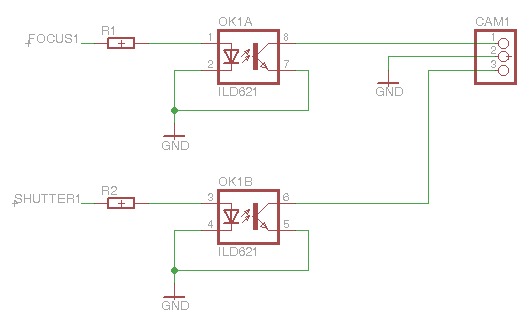
\includegraphics[width=0.5\textwidth]{singleopto}
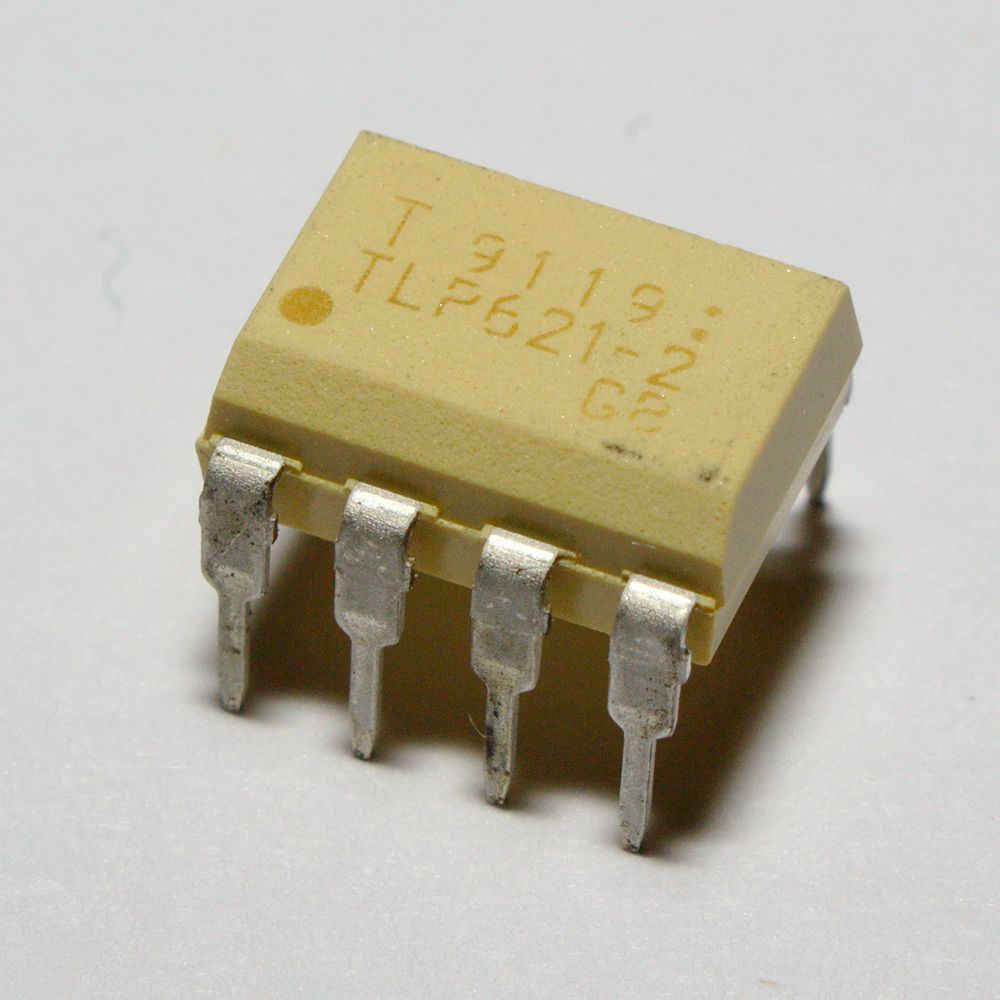
\includegraphics[width=0.3\textwidth]{tlp621-2}
}{fig:singleopto}{
	Left: schematic diagram for a single opto-isolator pair for shutter and focus of a camera, including the current-limiting resistors and a pin header connector for the camera signals.
	Right: TLP621-2 dual opto-isolator in a DIP8 through-hole package, with physical dimensions of approximately 10 by 7 mm.
}

\simplegfx{p}{0.8\textwidth}{triggerboard}{
	Final version of the printed circuit board layout for the trigger box.
	Full schematic available in the appendix. \ref{app:fullschematic}
}

\simplegfx{p}{0.8\textwidth}{camsremote-proto}{
	Remote trigger tool prototype on a solderless breadboard.
}

\simplegfx{p}{0.8\textwidth}{camsremote}{
	Remote trigger tool in a case, with lid removed.
	The left side includes buttons, indicator lights and a USB connector; the camera connectors are on the opposite side.
	The microcontroller board is attached to solderless connections, so that it can be removed later for testing purposes if necessary.
}

\subsubsection{Code}

STMicroelectronics advertises the Mbed programming environment and library for the board as an option for writing software for the MCU. \cite{mbednucleo}
The toolchain that compiles the binary for the board works also via the browser in a cloud service, but the libraries can be also installed locally.
All MCU-side code was developed using the Mbed libraries, built locally with the GCC-ARM Embedded toolchain \cite{launchpad-gcc-arm}.
Mbed hides the hardware complexity of the platform, making the total application source code small (less than 200 lines of C++) and relatively independent of hardware initialisation details.
A significant advantage in this hardware abstraction is that a novice could extend the program without previous knowledge on the particular hardware architecture.

The MCU software, or \emph{firmware}, communicates via a serial line that the board passes through USB as a standard virtual serial port, requiring no special drivers.
Communication protocol consists of flags for setting focus or shutter mode and entering bit flags that describe what cameras should be affected, in text mode.
The device echoes the sent characters back, making it convenient to test with a serial console.
The protocol is described in detail in table \ref{tab:triggerprotocol}.

The code also monitors the Nucleo's integrated general-purpose pushbutton that is used to focus and trigger all cameras simultaneously.
One press focuses all cameras, and subsequent presses send a short shutter signal.
The reset button resets the whole microcontroller, restarting the program with no focus or shutter signals selected.

\begin{table}[h]
	\centering
	\begin{tabular}{l l}
		Set focus pin state & Fxxxxxxxxxx\\
		Set shutter pin state & Sxxxxxxxxxx\\
		Reset all to unpressed & R\\
		Example: push down focus on first and third & F101\\
	\end{tabular}
	\caption{
		Remote trigger protocol; the letter x signifies a single bit (digit 0 or 1) and can be omitted from the start, in which case it is assumed 0.
		Note that the messages set the whole button state instead of sending ``keypresses'';
		to emulate a full keypress, the state must be set first to 1, followed by a set to 0 or a reset.
		Each command must be finished with a space or newline character.
	}
	\label{tab:triggerprotocol}
\end{table}

The used Mbed library does not actually turn all pins on at exactly the same time but in fast succession.
This is not a problem because of the high clock speed of the processor;
the difference between first and last pin changes was measured to be a negligible 1,6 microseconds.
%Expected variance from each camera is supposed to be orders of magnitude longer.

Control software for the host PC was implemented as a small command-line Python script communicating to the virtual serial port of the Nucleo board.
The host controls the trigger's outputs individually, normally driving all the outputs at once.
Sequential or other forms of triggering are possible, because the cameras are controlled individually in hardware.
For example, as each camera is able to record five full-resolution frames per second in burst, interleaving the nine cameras results in short 45 FPS full-resolution imagery.
Also, when using the internal pop-up flashes in the cameras, they can be fired separately to circumvent issues in lighting synchronization or exposure control.

The same MCU can be reprogrammed with another firmware at any time; it was used also for measuring shutter delay of one camera, see section \ref{sec:shutterdelaymeas}.

The programs are available in \url {http://github.com/sooda/thesis} with source code.

% }}}

\subsection{Custom camera control software} % {{{

% breeze systems $129 per cam
% smartshooter

% FIXME clumsy
% esper design etc.
%General parallelized image acquisition from a large set of cameras has not yet established such a state that general purpose software would be easily available.
%Commercial solutions probably exist, but they are often strictly bound to a specific hardware, expensive, and inflexible.

Some custom techniques were used to preview images of all cameras simultaneously, configure the settings of each concurrently, and retrieve the captured images from them in order.

Like the MCU board layout and firmware, all programs and their sources can be downloaded from \url {http://github.com/sooda/thesis}.
The programs have been verified to work under recent Linux and Mac OS X systems.

% }}}

\subsubsection{Camera control library} % {{{

\paragraph{Camera libraries}
gPhoto2 \cite{gphoto2} is a well-known free and open-source application and library in the C programming language for controlling digital cameras on Unix-like operating systems, supporting over a thousand cameras.
The software consists of a command-line control tool of the same name, \emph{gphoto2}, and a library API, \emph{libgphoto2}.

Instead of relying on each camera manufacturer separately for a software development kit, gphoto2 abstracts common operations behind the same interface.
For example, Canon and Nikon, some of the biggest camera manufacturers, both provide SDKs for controlling their devices remotely via a USB connection from Windows and Mac OS X. \cite{canonedsdk} \cite{nikonsdk}
Sony provides an SDK for Android and iOS. \cite{sonysdk}
Olympus has had an SDK, but it is no longer available. \cite{olympussdk}
To support all vendors, one would have to write code for all APIs.
In this work, extendability to other vendors was seen as an optional advantage.
In addition, development kits provided by the vendors may be more restrictive and may not be fully available.
%Canon provides a Digital Imaging Developer Programme that requires registration to be able to download the SDK (EOS Digital SDK, or EDSDK).

Furthermore, the Canon EDSDK claims in the manual not to support sessions to more than one camera in parallel. \cite{canonedsdk}
This technical issue could probably be overcome with additional workarounds in software, though.

Libgphoto2 implements the \emph{Picture Transfer Protocol (PTP)} \cite{ptpTODO} for setting properties and transferring pictures via USB.
Details on list of configurable properties and sequences for capturing pictures and preview vary among manufacturers, and the library has most thorough support for Canon and Nikon cameras.

\paragraph{gphoto2 wrapper}
A ``wrapper'' code library was written in C++ for libgphoto2 to automate memory and resource management, simplify the usage of the raw library, and to write the programs themselves in clean C++; libgphoto2 itself is implemented in the C language and is not well documented.
Libgphoto2 exposes the data as objects, and the wrapper simplifies their handling and implements some more complicated operations, such as creating a new camera object instance, configuring parameters, and downloading preview frames and actual shots.
The library itself is also not thread-safe: if a camera is used in to threads of execution simultaneously, unexpected errors happen. \cite{gphoto2}
Locking mechanisms were written for the wrapper to prevent more than one executing threads from accessing a camera instance simultaneously.
The library initialization was also protected, because it loads camera-specific sub-libraries only after first use; if many cameras are tried to initialise at the same time, another error would occur.

The wrapper is written exclusively with libgphoto2 in mind, but as it actually hides the implementation details strongly, it could be ported to use e.g. EDSDK without affecting the actual applications using it.

% }}}

\subsubsection{Previewing} % {{{

\simplegfx{h}{1.0\textwidth}{gphotogrid}{
	A custom program, \emph{gphotogrid}, was written for displaying a preview feed of many cameras in a grid and configuring exposure time, aperture, and ISO sensitivity jointly for all cameras.
	New settings are easy to add if needed.
}

\simplefig{h}{%
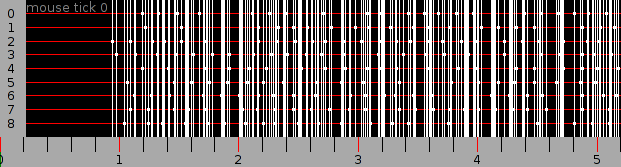
\includegraphics[width=\textwidth]{timeline-nosync}
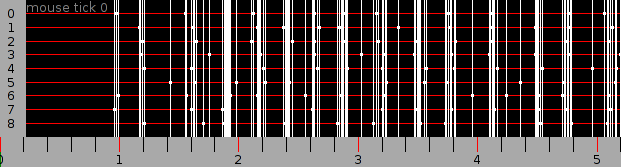
\includegraphics[width=\textwidth]{timeline-sync}
}{fig:grid-timelines}{
	Timelines displaying the points in time (x axis, in seconds) when frames have been captured from different cameras (y axis, by camera number).
	The upper image shows all cameras running freely, and in the lower image, no new frame is captured from any camera until all have finished the current capture.
}

Although each camera can be positioned by individually looking through the viewfinders, a simple preview live feed is almost mandatory to properly set up a new configuration to see the big picture.
A preview matrix of all cameras makes it easy to identify the cameras and to see if they all have been pointed to correct directions, and to verify that their settings are the same by judging from the image quality.
The program is shown in Figure \ref{fig:gphotogrid} and is found in the github repository under the name \emph{gphotogrid}.
It is written in C++ and uses the libgphoto2 wrapper for camera control and the wxWidgets GUI library \cite{wxwidgets} for the user interface.
The purpose is to view the picture frame of each camera in realtime and change the most important camera parameters concurrently.

\paragraph{Preview stream}
Libgphoto2 provides an interface for reading a camera preview frame at a rate of several frames per second, speed depending on USB hardware performance, the number of cameras used in parallel because of USB bus limits, and CPU processing power as the images are resized to the screen.
A preview feed is connected to each camera to download the frames as fast as possible, and the user interface displays them as a grid, with configurable camera order.
Because libgphoto2 does not offer asynchronous image or configuration transfers, a new thread of execution is set up for each camera, and the preview pictures are transferred to the main screen via concurrency-safe queues in the application itself.

% FIXME this to experiments?
\paragraph{Timeline}
A timeline widget was also developed to investigate the points in time when the preview frames have been grabbed, aiming to study synchronization accuracy using this preview method.
Observing the times was found to be of no use, because the pipeline from camera to application seems to be so complex that the preview frame rate is completely sporadic, with no ability to control the frame order or timing.
The application includes a checkbox for ``synchronizing'' the preview grabber threads so that no camera starts to read a new preview before all have read the last frame.
This synchronization attempt did not have any positive effect; in contrast, restricting each camera this way made the performance much worse, as can be seen in Figure \ref{fig:grid-timelines}.
In the figure, a vertical bar is drawn for each frame captured, with a small circle on the line of each corresponding camera number.

\paragraph{Identification}
The cameras are identified and ordered by a name written to the configuration set under a property called \emph{artist}, found at least in Canon DSLRs.
The artist name can be set either via USB or from the camera's physical user interface, and it is supposedly originally meant for writing the camera owner's name in the image file's metadata, along with copyright information.
For the camera rig, a single letter was used for each camera, ordered from \emph{A} to \emph{I}.
A separate configuration property stored in the camera itself is most robust; USB port name can be used as an alternative to identify the cameras, but the port name changes when the cameras are plugged in another way when rebuilding the rig or using another computer.

The pop-up flashes should not be activated during use, because the camera was found to ignore the effects of most settings when the flash is up.
Additionally, remote control disables the camera user interface.
Taking pictures or changing settings is not possible while previewing.

It is recommended to spread the cameras as evenly to all USB root hubs as possible to help even out the transmission capacity, maximizing the frame rate.
The same is recommended when downloading the actual images.
The USB hub where a device is connected can be verified in Linux by looking at the output of the \emph{lsusb} command-line tool.

% }}}

\subsubsection{Configuration} % {{{

Remote control of all cameras is required to set all settings, such as shutter speed, jointly from the same computer instead of clicking on each camera's buttons manually.
The preview matrix program allows to change exposure time, aperture size and ISO sensitivity, but more tools were written for automatic configuration.

The following small command-line scripts were written using the gphoto2 command-line tool:

\begin{itemize}
	\item \emph{config}: reset common parameters to defaults for all connected cameras, listed in the script itself
	\item \emph{forall}: run gphoto2 with the user supplied arguments for all connected cameras serially
	\item \emph{forallp}: as forall, but in parallel, saving time
	\item \emph{post-download-by-camid}: download all previously shot files stored in the cameras to directories named by camera artist name
	\item \emph{readconfig}: read and copy settings from one camera to all others currently connected
	\item \emph{release-uilock}: unlock the physical user interface of connected cameras by fetching a listing the filesystem; a workaround for the Canon glitch described below
\end{itemize}

The \emph{forall} and \emph{forallp} scripts are trivial shortcuts to autodetecting all cameras and passing commands to gphoto2 for each, and are useful for case-specific problems or e.g. setting individual configurations temporarily.

With \emph{readconfig}, one camera is first configured manually, and the settings are cloned to others automatically with the script.

Either libgphoto2 or the EOS 700D camera has a bug that locks the camera's physical user interface when configuring the cameras and even quitting the program:
it appears that this is a safety feature that is left on after disconnecting the configuration connection, and probably gphoto2 does not release it properly.
When setting or getting any configuration, the camera screen turns off and all buttons stop responding until the camera is rebooted, USB cable is unplugged, or if gphoto2 touches the camera's filesystem.
Listing the files is thus enough and it has no side effects.
The workaround script \emph{release-uilock} was written as a reminder to perform the listing for all connected cameras.

% }}}

\subsubsection{Image acquisition} % {{{

% offloading

A command-line tool called \emph{paraphotos} for downloading the images in realtime in parallel from each camera was developed in C++ using the same libgphoto2 library wrapper.
The cameras send a notification when a new photo is taken with the shutter button or the remote release.
When this new file is found, it is downloaded and named by a running index and camera name.
The user is notified when all cameras have finished for a single shoot;
also, when the program is requested to quit, it first waits until the last pending download is finished.
Each download task runs in a separate thread of execution to overcome the synchronous nature of libgphoto2, as well as the notifying task; Figure \ref{fig:img-get-process} depicts simplified code control flow.

\simplegfx{h}{0.8\textwidth}{img-get-process}
{FIXME: this is ugly. Simplified flow graph of the paraphotos program control flow.}

Almost the same functionality could have have been achieved with the gphoto2 command-line utility; using the library directly with C++ resulted in cleaner code and probably faster operation.

Video acquisition is not possible in realtime; instead, the video files have to be saved on the memory cards first, and downloaded when the recording is complete.
The \emph{post-download-by-camid} clones the file systems from the cameras to local disk, bringing the video files accessible.

Video format should be set to 720p at 50 or 60 FPS or 1080p at 25 or 30 FPS.
Both resolutions result in a video bitrate of approximately 5 MB/s with default settings.
The video format is H.264 encoded in a Quicktime MOV file, with a stereo audio in raw lossless (PCM) format with 48 kHz sample rate and 16 bits per sample.

The bitrate can be extended from Magic Lantern's menus, but bitrate changes are still experimental code and recording may stop if the camera or the memory card is not fast enough.
Video keyframe rate can also be changed with a development version of ML and probably will be stable in the future;
in the video codec used, the frames can be \emph{I-frames} (intra-frames), with fully encoded data, or \emph{predicted frames}, encoding changes between frames, with less accurate information.
Raw recording is also supported, but with the limited memory card speed, only a low resolution is achievable.

% }}}

\subsection{3D reconstruction software survey} % {{{

% something on individual algorithms/tasks of the reconstruction pipeline; standalone pipelines; web services; sw/hw solutions

When the imagery has been downloaded to a PC, the actual reconstruction can be started.
There is a wide collection of libraries, open-source tools and commercial packages for both automatic reconstruction and generic mesh editing for post-processing the data.
Some of them are presented in this section.
In the scope of this work, new reconstruction algorithms or implementations are not implemented;
thus, it is important to test the rig with readily available implementations.

Many, if not all, programs assume that the Exif data embedded in the photograph files describes the used focal length and sensor dimensions.
Canon EOS 700D stores this information properly in the files.

 % }}}

\subsubsection{Free libraries} % {{{

There exist several generic computer vision and geometry and image processing libraries, most common of them being probably OpenCV \cite{opencv}, Point Cloud Library (PCL) \cite{pcl} and Computational Geometry Algorithms Library (CGAL) \cite{cgal}.
These are written in the C and C++ languages and they have bindings to several scripting languages too.
For future work using the rig, these libraries present a well known basis for developing own tools.

OpenCV contains a large set of utilities for 2D image processing and extends also to camera calibration and 3D reprojection.
It is probably the most commonly known and most used computer vision algorithm package.

PCL contains a set of algorithms for filtering, segmentation, registration, visualization, and more for working on data sets that consist of points that may share attributes such as colors and normals.
PCL is popular in robotics involving three-dimensional computer vision; its algorithms apply well to point cloud data obtained easily using a LIDAR or similar range imaging device.

CGAL provides access to more general and mathematically more geometric data structures and algorithms extending in combinatorics, convex hulls, polygons, arrangements, mesh processing, triangulations, voronoi diagrams, visualization and more, with a more mathematically rigorous approach.

% }}}

\subsubsection{Free programs} % {{{

While libraries can be used to write new tools, many pieces of software are readily available that implement 3D reconstruction based on methods presented in Section \ref{static3d}, and are distributed in source code form and/or readily usable binary executables.
Some of the most known state-of-the-art implementations are listed below.

Camera Calibration Toolbox for Matlab, also included built-in in OpenCV, is a more or less standard tool to single-camera and stereo camera calibration.
The toolbox computes undistortion maps and intrinsic and extrinsic parameters with checkerboard images using non-linear optimization and planar homographies. \cite{camcalmatlab}

Bundler is a bundle adjustment and structure-from-motion system for computing camera poses and sparse point clouds, targeted for large-scale unordered photo collections, originally used for the Photo Tourism project. \cite{snavely2006photo}

SiftGPU is a fast SIFT implementation for graphics processing units (GPUs) by Chenchang Wu. \cite{changchang2007siftgpu}
It is built on Sift++ \cite{vedaldi2011sift++}; both are based on difference of gaussians, a method for edge detection. \cite{marr1980theory}

Multicore (parallel) bundle adjustment PBA is a fast bundle adjustment library built with the modern parallel nature of multi-processor computers in mind. \cite{wu2011multicore}

Patch-based, multi-view stereopsis (PMVS) starts from a set of matching keypoints (features) and a pre-acquired camera calibration, and expands the keypoints to a dense patch set iteratively, resulting in a high number of oriented points.
PMVS is usually combined with CMVS, a clustering tool that decomposes the input set to smaller clusters that are more convenient to process, when the amount of different views is large. \cite{furukawa2010accurate,furukawa2012patch}
% xxx viewpoint invariant patch, repetition analysis http://www.academia.edu/2021718/3D_Digitization_using_Structure_from_Motion
% xxx2 graclus, wat pba

VisualSFM \cite{wu2013towards} is a common and free but closed-source full-scale pipeline that implements a structure from motion algorithm and simplifies the workflow of several external programs, finally visualizing the results.
The needed external tools are feature matching, bundle adjustment and dense reconstruction.
VisualSFM is probably the most common tool in the open source and research community for practical use.
It integrates into a few clicks the pipeline from images to 3D point cloud, using SiftGPU for features, its own radial undistortion model and SfM for camera estimation, PBA for bundle adjustment, and finally PMVS/CMVS for dense matching.
A common final step is to use Meshlab to filter outliers away from the data and to build a triangular textured mesh of it with the input points and normals.
%PMVS is suggested by many others.

Meshlab \cite{meshlab} is a generic interactive editor of point clouds and meshes, implementing many scientific papers.
It can be used interactively and scripted to do the same steps automatically.
In a reconstruction pipeline, it is one of the last processing steps, used for removing outliers or fitting a surface on a point cloud with the poisson surface reconstruction method, and finally projecting the textures to the generated mesh when given the camera parameters in relation to the point cloud pose.
It can also perform registration between point clouds.

(Screened) poisson surface reconstruction, or PoissonRecon, is another stand-alone program as an alternative for surface fitting. \cite{kazhdan2013screened}

Cmpmvs is a multi-view reconstruction software for transforming a set of calibrated image data to a full textured mesh, used in a similar way as VisualSFM but using internally a different method based on graph cuts and weakly-supported surfaces.
\cite{jancosek2011multi}

Python Photogrammetry Toolbox, popular in archaeological fields, combines Bundler and PMVS/CMVS for a full-scale pipeline. \cite{moulon2011python}

%SFM toolkit combines Bundler and CMVS/PMVS.

% }}}

\subsubsection{Commercial solutions} % {{{

There is a large selection of commercial software available, often accompanied with a 3D scanning device or a complete service.
Some companies offer completely specialized rigs, some sell a scanning device and a general-purpose software alongside it which can be used as standalone and some only sell software, leaving the hardware implementation to the user.

% FIXME emphasis on differences

\begin{description}
	\item[Autodesk 123D Catch] is a free and popular web-based application for automatic reconstruction; photos are uploaded to a cloud service, and a textured mesh is generated automatically. \cite{autodesk123dcatch}
	\item[Agisoft PhotoScan] has two editions, for 3D designers and professional geographic content manipulation; among the geographic features, it is very suitable for multi-view reconstruction in content generation, and has an active forum for its users. It can be scripted with the Python programming language. \cite{photoscan} Photoscan is used by \cite{ir-ltd}.
	%\item[CaptiveMotion] provides a facial capture and retargeting system that can be used with full-body mocap.
	\item[MotionScan] is the technology behind e.g.\ the video game L.A.\ Noire \cite{rockstar2011noire}, developed by CaptiveMotion. It uses tens of cameras to recover detailed structure and is targeted for video game content generation.
	\item[Faceshift] provides a realtime markerless face capture in a feature space that describes virtual muscle and bone movements, using a single camera and pre-trained poses. \cite{faceshift}
	\item[3DF Zephyr Pro] is an automatic reconstruction software that takes photographs as input. A free SfM software, \textbf{3DF Samantha}, is provided too. \cite{3dfzephyr}; The company (3DFlow \cite{3dflow}) is a spin-off of a university thesis project. \cite{toldo2013accurate,toldo2013towards}
	%\item[Mova Contour Reality Capture] does high-performance surface capture with a large array of cameras.
	\item[Pendulum Studios] provides a capture system called Alter Ego that integrates with game engines. \cite{alterego}
	\item[Pix4dMapper] converts aerial images to geometric surface models. \cite{pix4d}
	\item[Acute3D] Smart3DCapture is targeted for large-scale photogrammetry and cultural heritage digitization. \cite{acute3d}
	\item [FARO] manufactures hardware and provides scanning software for 3D documentation and surveying, and provides a free application for Kinect-based scanning. \cite{faro}
	%\item[Trimensional] is a 3D scanner for iPhone.
	%\item[Fuel3D] is a complete low-cost handheld scanning system.
	\item[Dimensional Imaging ltd.] provides DI3D and DI4D systems and software for static and dynamic surface capture, respectively. \cite{di4d}
	%\item[SynthEyes] 
	\item[Pixel Farm] provides tools for reconstruction, CG integration and match moving. \cite{pixelfarm}
	\item[3D-equalizer] is a multi-platform 3D tracking solution for the visual effects industry. \cite{3dequalizer}
	%\item[V-STARS] by Geodetic System has emphasis on 3D measurement and engineering.
\end{description}
% ms photosynth

% TODO vicon; bradley face capture explains some.

%\subsubsection{Other}

%- voodoo camera tracker
% cyberware no longer exists, was used in films in hollywood
%- canoma no longer
%- bundler based on photosynth?
%- janimation head tech
% - KLT: http://www.inf.ethz.ch/personal/chzach/opensource.html
% http://slowmovideo.granjow.net/

% }}}

%\subsection{Sample reconstruction pipeline} % {{{
%%\subsection{Full reconstruction} % {{
%
%Both shape and texture are considered in this work. Only diffuse color (albedo) is of interest; more complex material properties are assumed to be captured in other means and not spatially varying.
%
%Basic uv mapping. Project texture to computed mesh. Somehow use colors and optical flow everywhere...
%
%Postprocessing: remodel the mesh (face), see what it would look like. Refine parameters to get a similar output as in the photos (normal map etc.), backproject. Use colors and highpass them; assume uniform lighting and locally uniform texture color (bradley). (Simply a rendering technique, that level of detail in 3D structure might not be needed).
%
%facial expression space, faceshift, face muscles
%%
%%KINECT 2 HYBRID SHIT YEA
%%
%%eigenface / pca / AAM model (?)
%%
%%poisson surface vs ball pivoting
%%
%%visual convex hull, bbox for constraining
%
%% }}}
%
%\subsection{Computer requirements} % {{{
%
%any pc with usb and linux/mac/?? will do, the bigger the better
%
%% }}}

